\begin{savequote}[8cm]
\textlatin{Neque porro quisquam est qui dolorem ipsum quia dolor sit amet, consectetur, adipisci velit...}

There is no one who loves pain itself, who seeks after it and wants to have it, simply because it is pain...
  \qauthor{--- Cicero's \textit{de Finibus Bonorum et Malorum}}
\end{savequote}

\chapter{\label{ch:7-com}Centre-of-momentum variables} 

    Inspired by the kinematic measurement of hadrons, I have constructed a set of new variables specific to the $\numuccopi$-Trackless sample and I call them the centre-of-momentum (COM) variables. 
    The key idea is to reconstruct the $\deltapp$ momentum using only hadronic variables.  

    The $\numuccopiop$ sample contains mostly resonance reaction, where the proton and the pion are the decay products of the $\deltapp$. 
    Without FSI, the sum, $\vecpsum$, of the proton momentum, $\vecpp$, and the pion momentum, $\vecppi$, is exactly equal to the $\deltapp$ momentum, $\vecpdel$. 
    Hence, if the proton and the pion are boosted back to the $\deltapp$ rest frame, the pion decay angle, $\pidecang$, with respect to the $\deltapp$ direction in the lab frame should follow the theoretical prediction. 
    However, with FSI effects, $\vecpsum$ would not be equal to $\vecpdel$ anymore. 
    Nonetheless, the hadrons can still be boosted by $-\vecpsum$, and certainly, the resultant distribution of $\pidecang$ would deviate from the theoretical prediction. 
    This deviation can serve exactly as an FSI probe. 

    It might seem similar to the Adler angle~\cite{ADLER1968189}, which is also a reconstruction of the pion decay angle. 
    However, the crucial difference lies in the reconstruction method of $\vecpdel$. For the Adler angle, $\vecpdel$ is reconstructed as the difference between the neutrino momentum, $\vecpnu$, and the muon momentum, $\vecpmu$. 
    The advantage of using the leptonic kinematics is that hadrons are conventionally harder to measure as suggested in Ref.~\cite{Sanchez:2015yvw}. 
    However, it has several shortcomings. 
    Firstly, $\pnu$ is unknown and can only be estimated from the final particles and hence the large particle kinematics uncertainty. S
    econdly, it assumes the struck nucleon is static, so it is also affected by initial nucleon motion. 
    In contrast, the hadronically reconstructed $\vecpdel$ is completely independent of the nucleon initial motion, thereby making the corresponding COM $\pidecang$ an excellent FSI-only probe. 

    Another variable of interest is the invariant mass of $\Delta^{++}$, $\mdeldec$ constructed from the hardronic variables.
    \begin{equation}
        \mdeldec=\sqrt{\esum^2-\psum^2},
    \end{equation}
    where $\esum=\epi+\ep$ is the sum of the pion energy and proton energy calculated in the lab frame. 
    Just like the $\pidecang$, without FSI, there is a theoretical prediction for the distribution of $\mdeldec$ which is closely related to the $\deltapp$  Breit-Wigner curve. 
    Any deviation from the theoretical prediction can only be caused by FSI, and thus, like $\pidecang$, $\mdeldec$ would also be an excellent nuclear model-independent FSI probe.

    The physical application of $\pidecang$ in FSI model discrimination is still under investigation, so only the reconstruction qualities of the COM variables are reported in Fig.~\ref{fig:1pi-com-res}. 
    Both $\pidecang$ and $\mdeldec$ can be reconstructed with excellent resolution, $2.5\degree$ and $6.0~\mevc$ respectively, thereby laying firm foundation for using these variables in subsequent physical analyses.

   \begin{figure}[!htb] 
       \centering
       \begin{subfigure}{0.45\textwidth}
            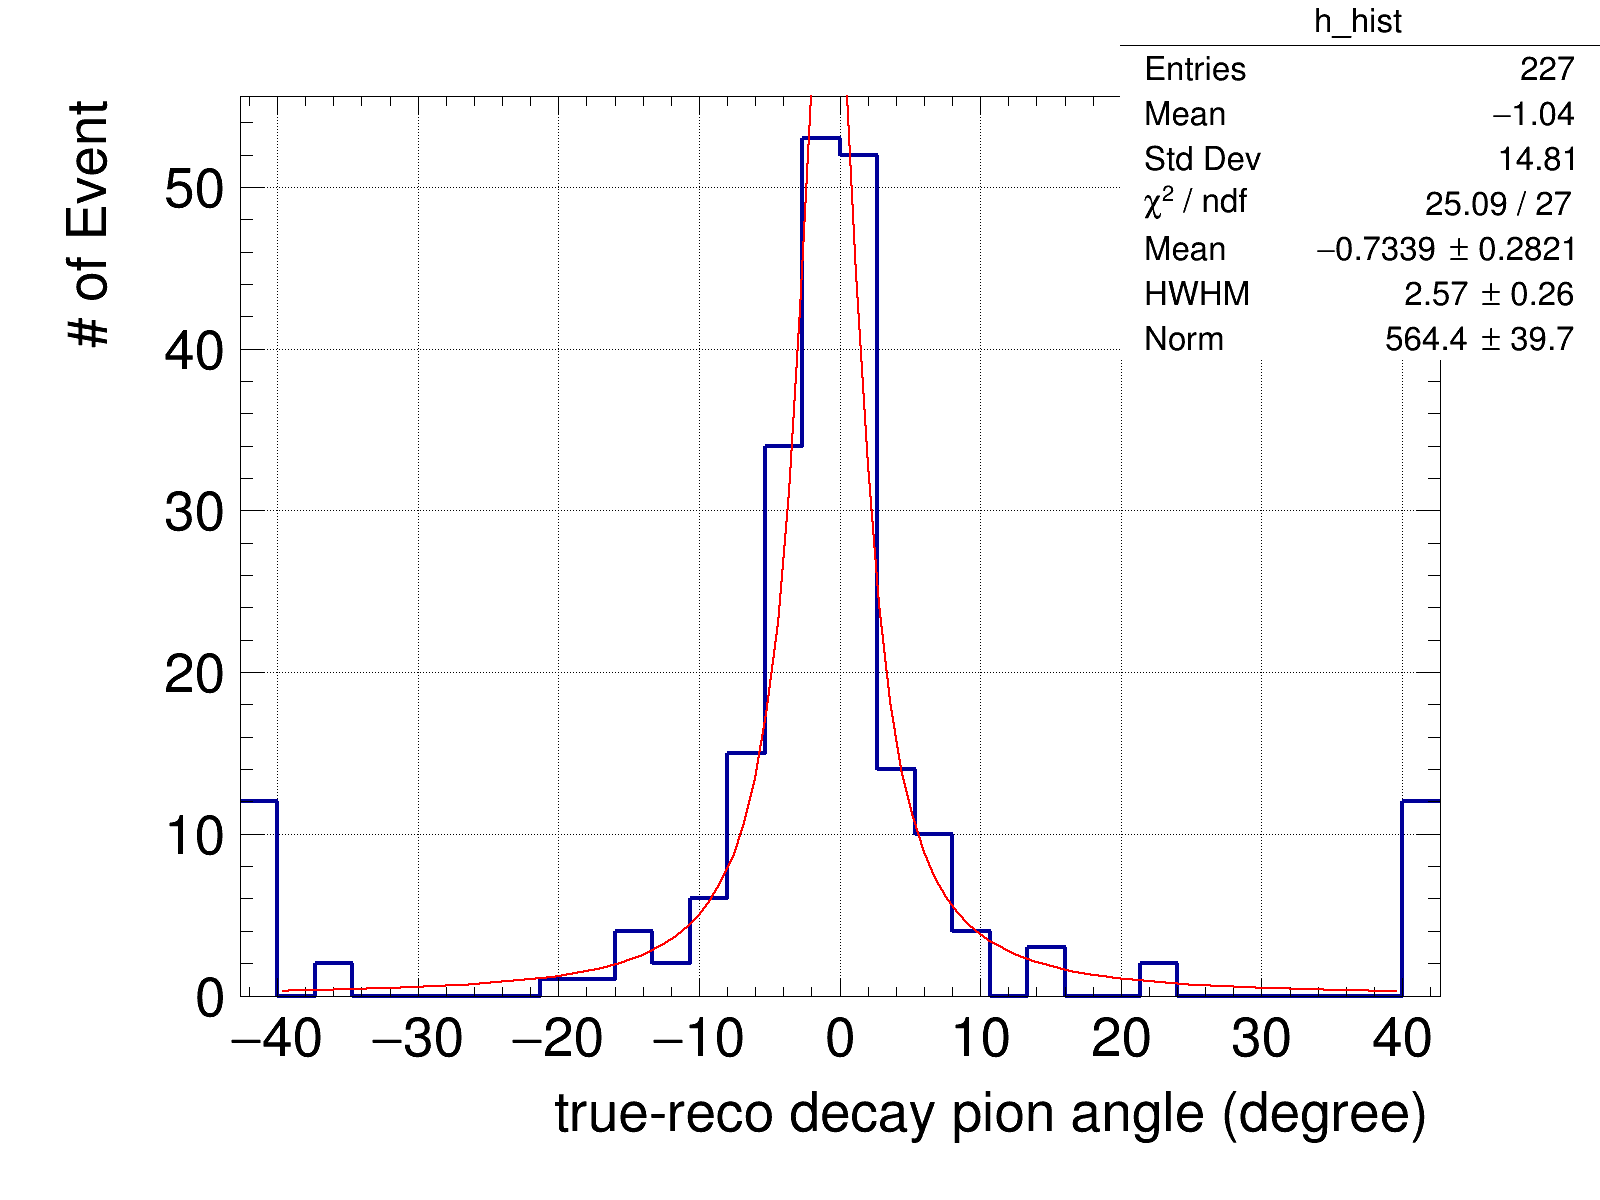
\includegraphics[width=\textwidth]{fig/SFGpTPCmu_dang_res_hist_al14.png}
            \caption{$\pidecang$ resolution.}
            \label{fig:1pi-decang-res}
       \end{subfigure}
       \begin{subfigure}{0.45\textwidth}
            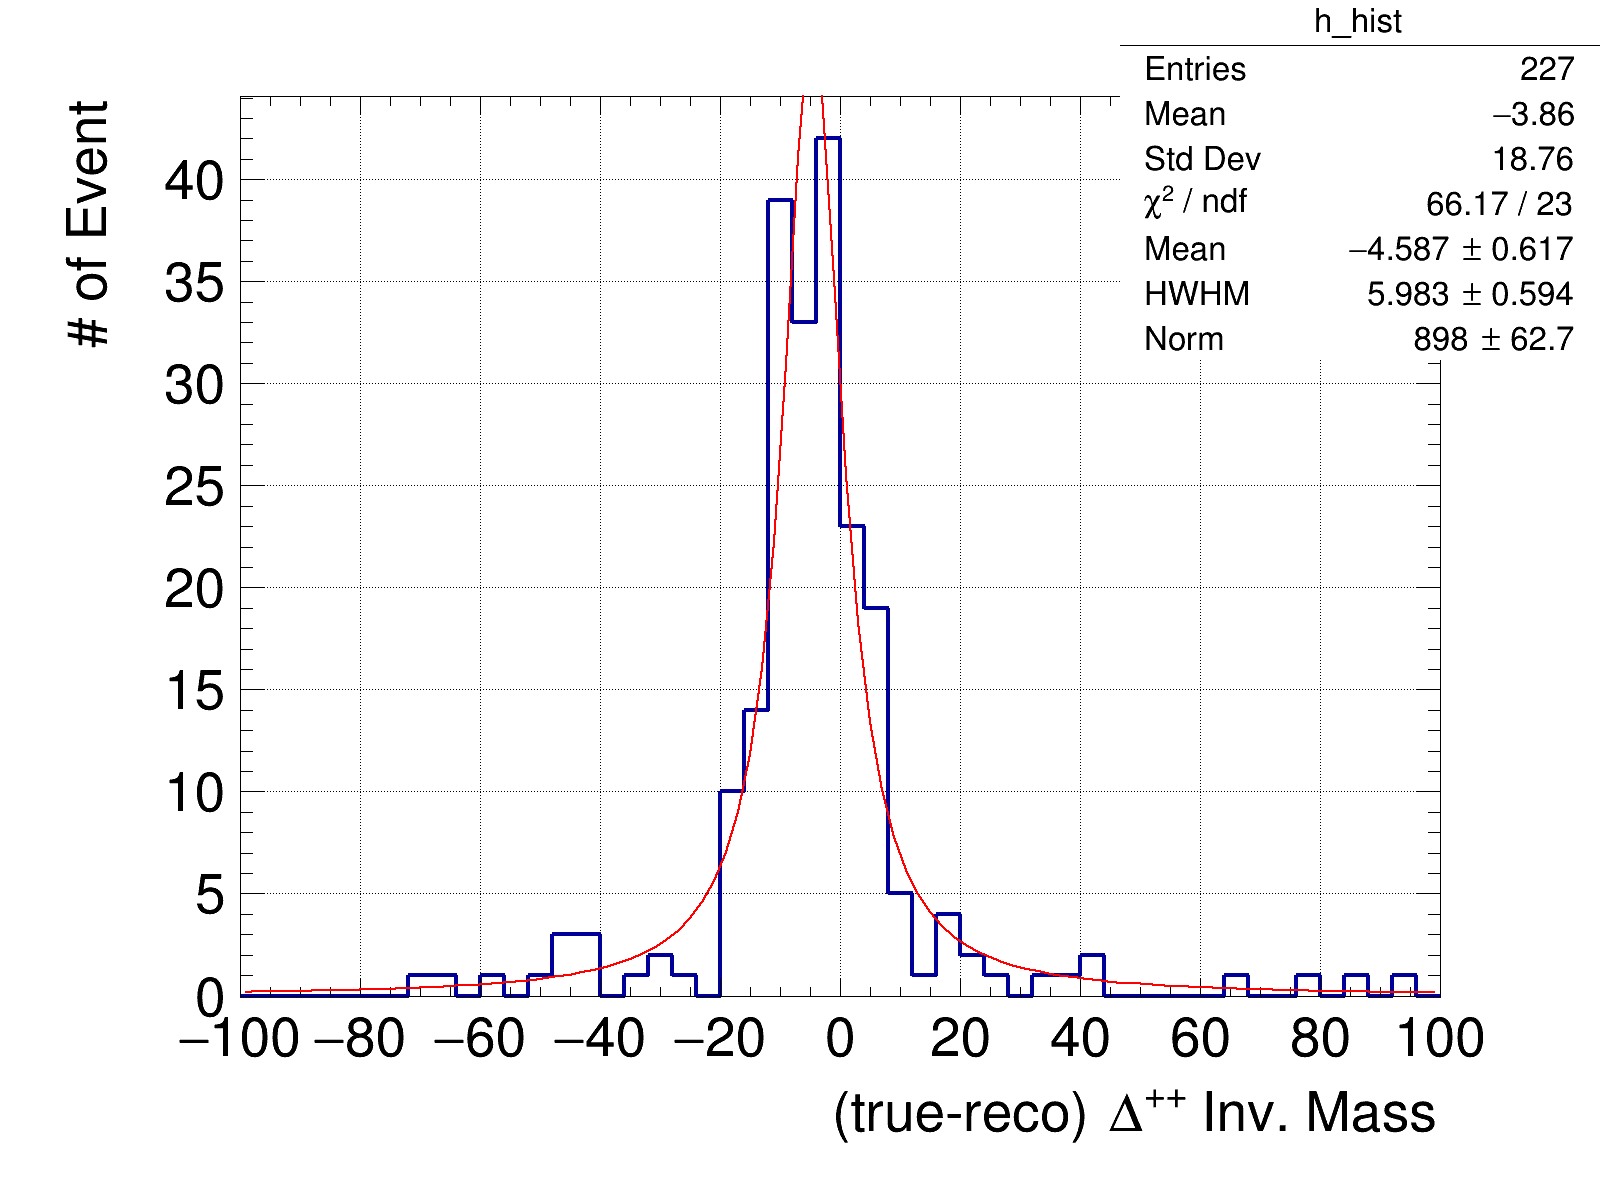
\includegraphics[width=\textwidth]{fig/SFGpTPCmu_edelta_res_hist_al14.png}
            \caption{$\mdeldec$ resolution.}
            \label{fig:1pi-mdel-res}
       \end{subfigure}
       \caption{COM reconstruction results.}
       \label{fig:1pi-com-res}
    \end{figure}
 

\section{Introduction}
There have been tremendous efforts to measure Charge-Parity (CP) violation in the neutrino sector by long-baseline experiments. 
Massive detectors, like Hyper-Kamiokande (Hyper-K) or the far detector of the Deep Underground Neutrino Experiment (DUNE), are proposed or being built. 
The measurement of $\dcp$, the CP violating phase, will have such large statistics that the uncertainties will be systematics dominant. 
It is pivotal to build more advanced models or to constrain existing models to provide more accurate predictions to maximize the physics potential of the coming experiments.
To gain a better understanding of the complicated neutrino-nucleus interactions, experiments with new and sophisticated detectors have started running, for example, the Tokai-to-Kamioka (T2K) experiment has upgraded the near detector and has started data collection in June 2024. 
Meanwhile, the Short-baseline Neutrino Detector (SBND) has also started running with a new ??? detector. 
These new detectors are much more capable than their predecessors. 
For example, the Super Fine-Grain Detector (SFGD) has a much-improved proton detection in terms of lower threshold, better resolution and higher efficiency. 
This advancement opens up possibilities for measurements of new useful variables. 
As the DUNE beamline ha a broad spectrum, it has a large contribution from resonance production, comparable to the quasi-elastic interaction.
Hence, it will be timely to explore new ideas with pions in the final states expecting the large influx of data. 

One effective method to improve our models is to constrain the parameters using existing data via tuning. 
There have been successful examples of observing better data-Monte Carlo (MC) agreement (cite cite cite) after tuning existing models using various combinations of measurement across experiments. 
However, as the neutrino-nucleus interaction is a convolution of multiple processes, namely the nucleon Initial State (IS), the neutrino-nucleon interaction and the Final State Interactions (FSI), many of the variables experience the impacts of all processes, thereby making it difficult to study the different models individually. 
Especially the nuclear effects, i.e. IS and FSI, are within the nucleus and cannot not be observed directly by present-day detectors. 
Hence, they contribute as a major source of systematic uncertainties. Cleverly construct variables, like the Transverse Kinematic Imbalance (TKI) (cite) variables or the Generalized Kinematic Imbalance (GKI), are sensitive to the nuclear effects. Past measurements have yielded fruitful model constraints [cite various TKI tuning paper]. 
While TKI is sensitive to both IS and FSI, new variables, like p_long [cite], are constructed to be particularly sensitive to a certain characteristic of the nuclear effects, in this case, the removal energy. 
Having more specialized measurement, like p_long, will be beneficial as it provides a more dedicated channel to fine tune our models. 

So far, all these variables are subject to both IS and FSI, except $\dat$, which is sensitive only to FSI but is affected by small uncertainties in the neutrino direction. As it is highly beneficial to have variables sensitive to a particular feature of the nuclear effects independently from others and in view of the enhanced detection capabilities and future measurements with pion in the final states. In this work, the author proposes a new set of variables, namely the centre-of-momentum (COM) variables in Charge Current Single Pion ($\ccopi$) events. The COM variables are capable of differentiating different FSI models regardless of IS models, thereby making dedicated studies on FSI possible. This work will elaborate on the concept of COM, followed by analysis results demonstrating the FSI differentiation power and the independence from IS. 

\section{COM}
When the neutrino possesses enough energy, it can excite the nucleon into a resonance, most commonly the $\deltapp$. This is the so-called resonance (RES) interaction. The resonance has a finite momentum from the RES interaction. However, it is extremely short-lived and decays quickly before exiting the nucleus, via 
\begin{equation}
	\deltapp \rightarrow \pip + \pr,
\end{equation}
as shown on the left in Fig.~\ref{COM-diagram}. The $\deltapp$ direction in the lab frame is chosen to be the x-axis, which coincides with the x’-axis of the $\deltapp$ rest frame. The angle, $\theta$, is defined with respect to the x-axis. As this is a two-body decay, the $\pdd$ can be obtained by summing $\ppi$ and $\ppr$, which can then be used to boost the system back to its rest frame. In this frame, the kinematics are exactly, given the rest mass of the resonance, except $\theta$ is chosen according to an underlying distribution, which are given by many models [cite MK etc]. 


So far the discussion on the resonance decay is completely general and hence it is applicable to and can be crosschecked by many other experiments, [hadron-nucleon collision?] There are properties specific to neutrino experiments. Firstly, the resonance is produced by neutrino interacting with a nucleon, so both vector and axial currents are present. Secondly, the interaction takes place inside the nucleus. This work explores the latter in greater depth, while the application of COM to the former will be pursued in future works. 


As the pion and the proton propagate out of the nucleus, they experience FSI, leading to modified kinematics, $\ppipp$ and $\pprp$, measured in the lab frame. Thus, the sum of measured momenta, $\psum = \ppipp + \pprp$, is in general not equal to $\pdpp$ anymore. Regardless, it is possible to boost the system to the centre-of-momentum (COM) frame using $\psum$, as shown on the right in Fig.~\ref{COM-diagram}. Similarly, $\thetap$ is in general different from $\theta$. In the absence of FSI, the COM frame coincides with the $\deltapp$ rest frame. Hence, the strength of FSI controls the extent to which $\ftp$ deviates from $\ft$. In practice, the measured $\ftp$ can be used as a probe to study FSI. Since the $\ft$ is a property of $\deltapp$ in its rest frame, it is independent of the $\deltapp$ momentum, and thus of the neutrino energy and of IS. Critically, $\ftp$ differs from $\ft$ only by FSI, which by definition is also independent of neutrino energy and of IS. As a result, $\ftp$ inherits these desired independences. 

FIG-COM-diagram

Conceptually, the COM angle might seem similar to Adler’s angle. However, there are key differences. Most importantly, the COM frame is reconstructed entirely based on hadron kinematics, while the Adler frame is built based on leptonic kinematics assuming stationary nucleons. Hence, the reconstruction of the Adler frame is affected implicitly by IS, while the hadronic variables are affected by FSI. Hence, Adler’s angle, a hadronic variable in the Adler frame, will be affected by both IS and FSI. Moreover, the need to reconstruct the neutrino energy makes variables in the Adler frame susceptible to the neutrino flux uncertainties, one of the largest systematics in neutrino experiments. [cite t2k result to prove]

To have a concise discussion on the main concept, this work focuses on $\deltapp$, as it is the dominant type from the T2K beam and it is also one of the most common types in DUNE [need to cite to prove both], but the idea is equally applicable to other resonances and implementations can be easily generalized. 

\section{Analysis result}
As there are no measurements of the COM angle yet, Monte Carlo studies have been performed to investigate its proclaimed advantages. Monte Carlo samples using \genie are produced using both the T2K and MINERvA beams and targets. Multiple \genie tunes are used in comparison. The model details for the different tunes are summarised in Table~\ref{tab:GENIE-TUNES}. Charge Current (CC) events with one pion and proton in the final states are selected to produce the plots.

TABLE:GENIE-TUNES



As shown in Fig.~\ref{fig:fsi-comp} (a), switching FSI on and off has a large impact on the $\tp$ cross-section measurement as expected. More importantly, Fig.~\ref{fig:fsi-comp} (b) demonstrates that a change of the underlying FSI model from hA (10a) to hN (10b) leads to a distinguishable shape change in the $\tb$ cross-section, thereby showcasing the FSI model discrimination power of $\tp$.

\begin{figure}
    \centering
    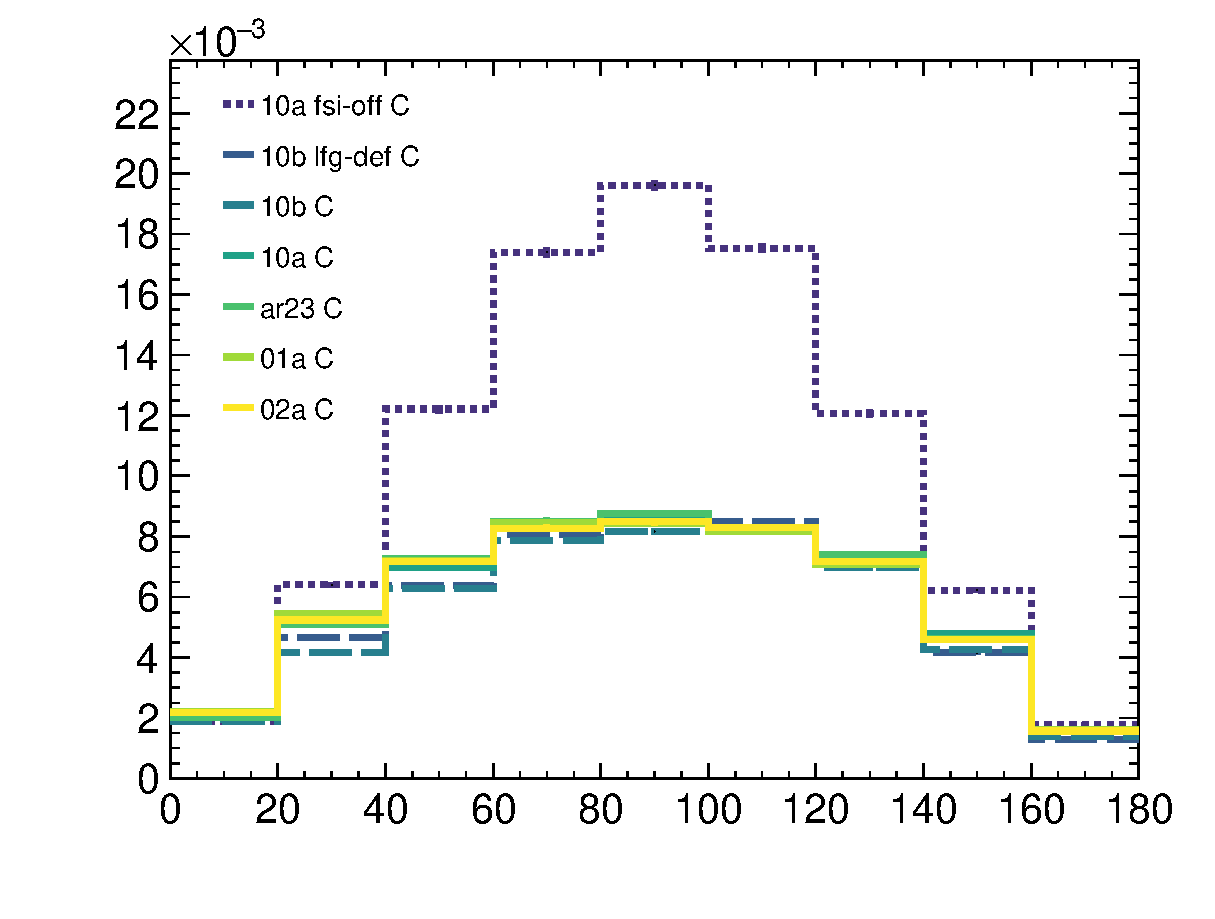
\includegraphics[width=\linewidth]{xnorm-mod-wfsioff-da.eps} \\
    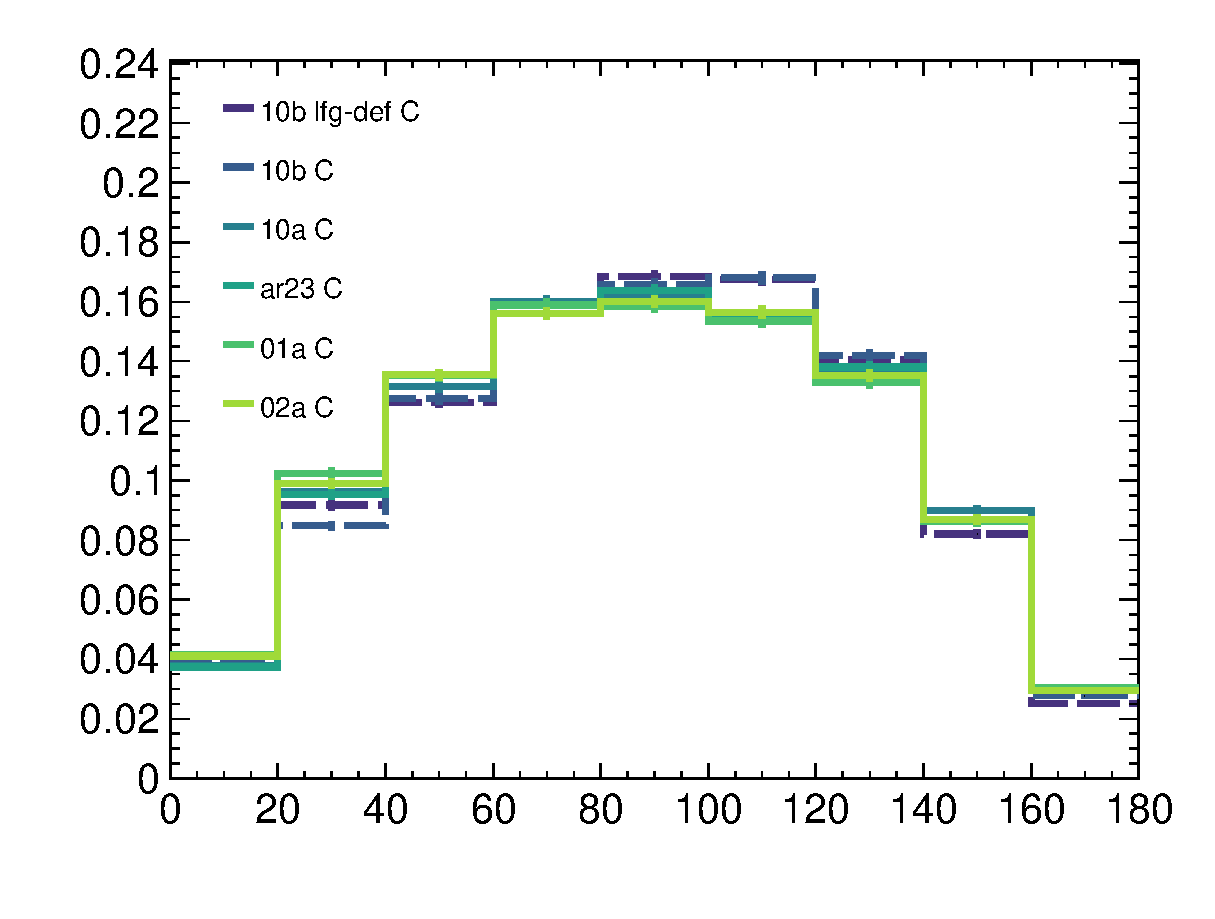
\includegraphics[width=\linewidth]{anorm-mod-nofsioff-da.eps}
    \caption{(a) Comparing FSI on/off xsec norm for 10a, (b) Comparing 10a and 10b (area normed)}
    \label{fig:fsi-comp}
\end{figure}

Another advantage of $\tb$ lies in its independence of IS. One ultimate test for this is to compare the cross-section shape of $\nu-C$ with FSI on and off with that of $\nu-H$. The $\nu-H$ interaction has no nuclear effect at all. The $\nu-C$ with FSI off shows the impact of IS, including removal energy for carbon and Fermi motion. The $\nu-C$ with FSI on has the full nuclear effects, both IS and FSI. As shown in Fig.~\ref{fig:ch-comp} (a), FSI has the strong impact on the cross-section shape as expected. The almost coincidence of the $\nu-H$ curve and the $\nu-C(fsi-off)$ curve is strong evidence supporting the claimed independence from IS of $\tp$.

\begin{figure}
    \centering
    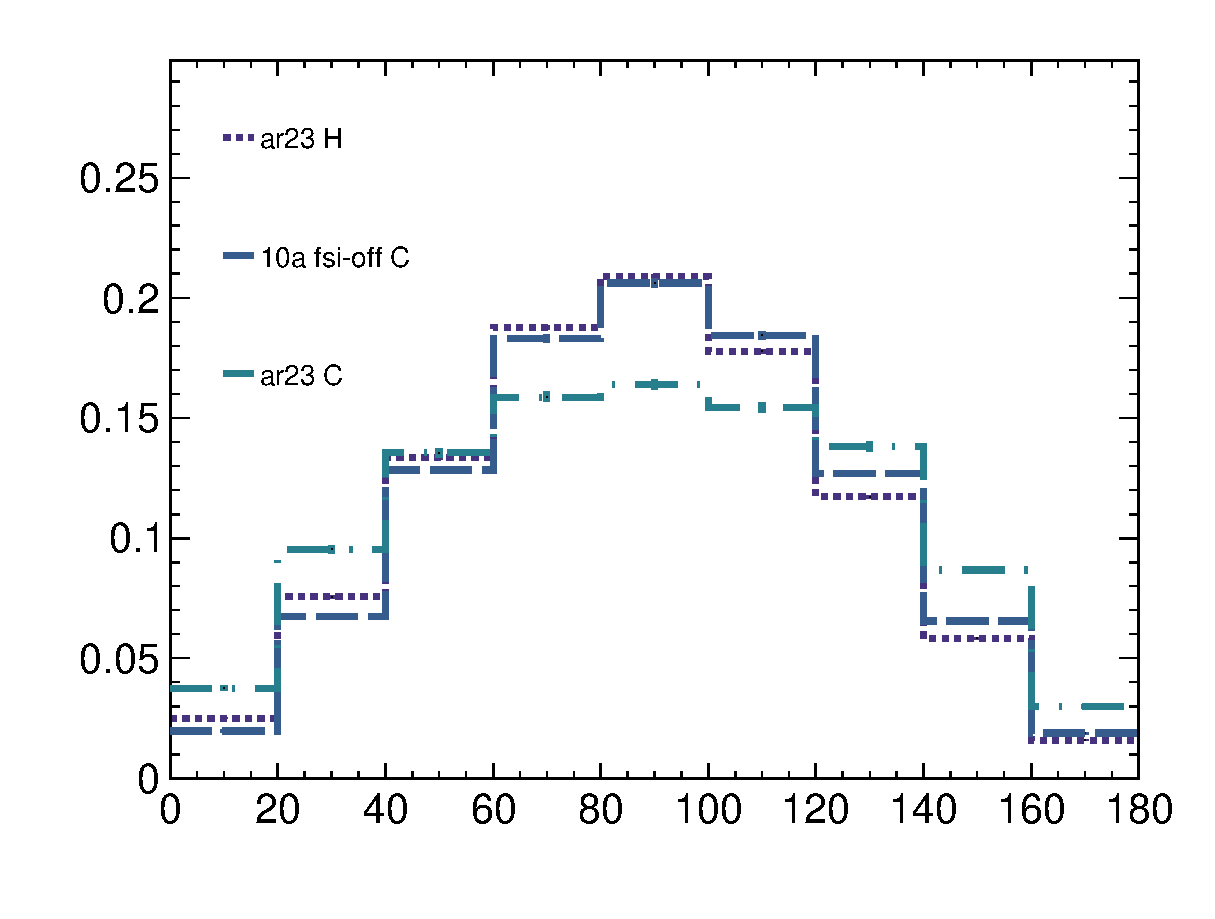
\includegraphics[width=\linewidth]{anorm-ch-da.eps}     \\
    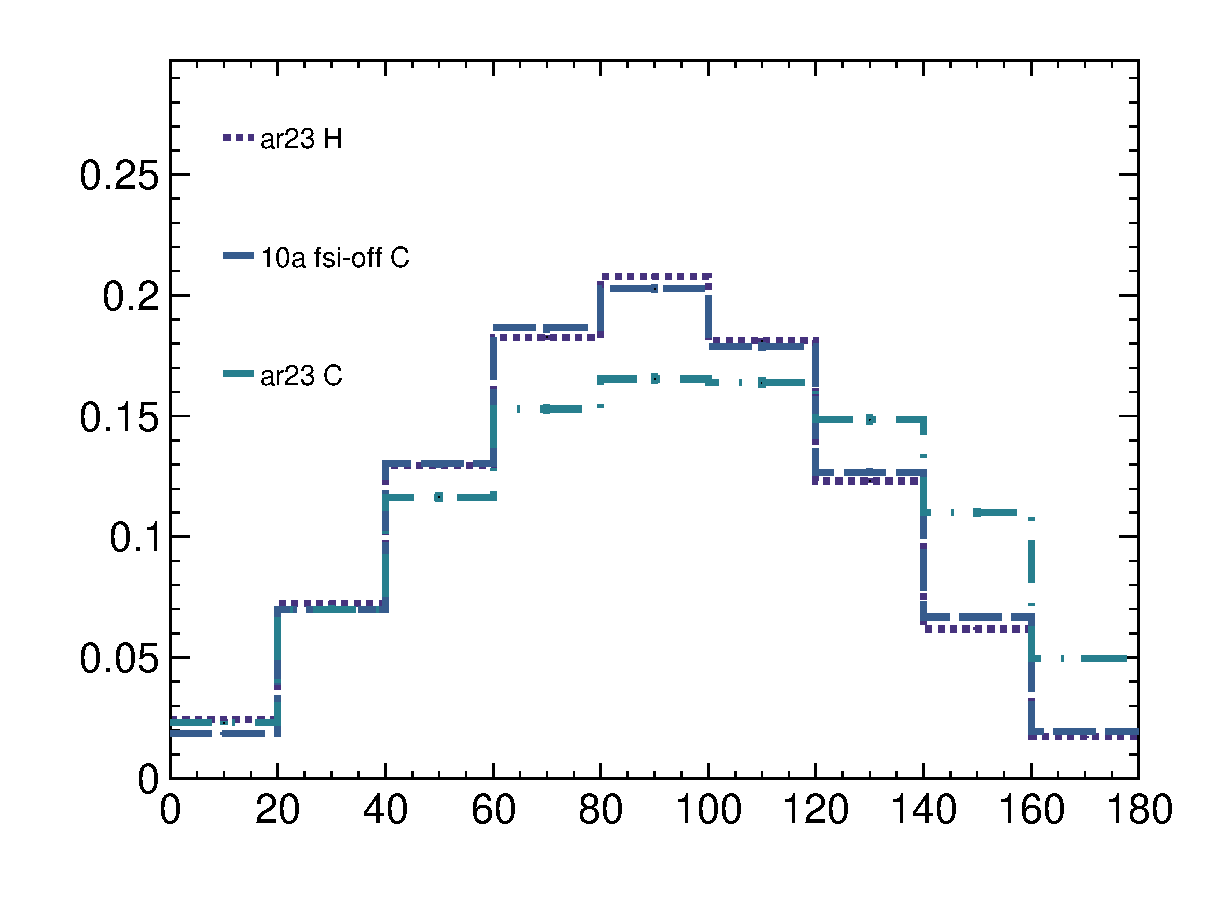
\includegraphics[width=\linewidth]{anorm-ch-adt.eps} 
    \caption{Anorm – nuH nuC(fsi-off) nuC(fsi-on) comparison. (a) $\tp$ (b) $\adt$.}
    \label{fig:ch-comp}
\end{figure}


Since $\tp$ is conceptually close to the Adler’s angle except that Adler’s angle has the additional influence from IS. In Fig.~\ref{fig:ch-comp} (b), the $\nu-H$ curve and the $\nu-C(fsi-off)$ curve are just as close to each other as in Fig.~\ref{fig:ch-comp} (a), suggesting that despite the dependence on IS, IS effectively does not distort the $\adt$ shape appreciably. This could put the claimed IS independence of $\tp$ in question, as it could be due to relatively small impact from IS. To verify this claim, a further stress test is performed. The removal energy of carbon is varied significantly, even to unphysical extents, to just observe its impact on the shape of $\tp$ and $\adt$. The result is shown in Fig.~\ref{fig:ermc-comp}.

\begin{figure}
    \centering
    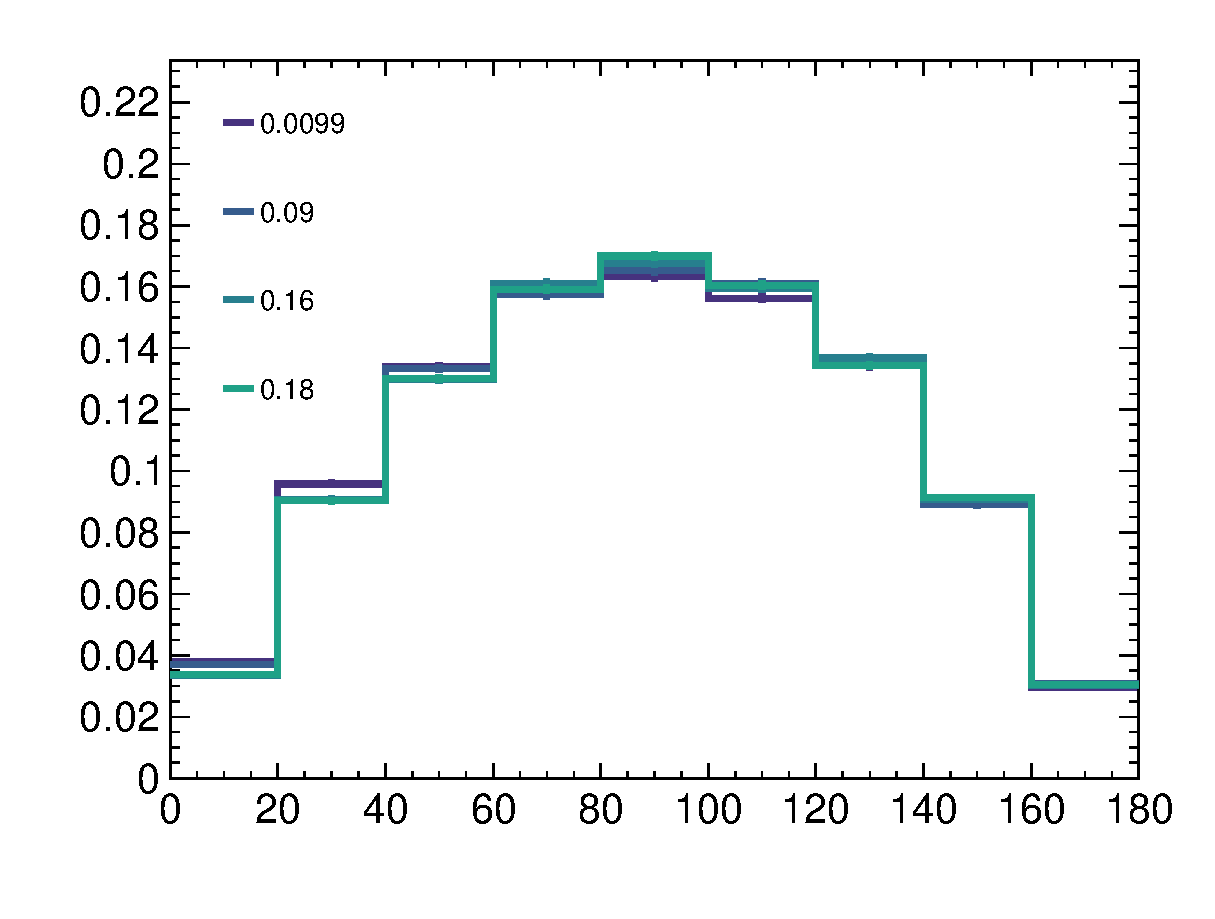
\includegraphics[width=\linewidth]{anorm-nuc-da.eps}\\
    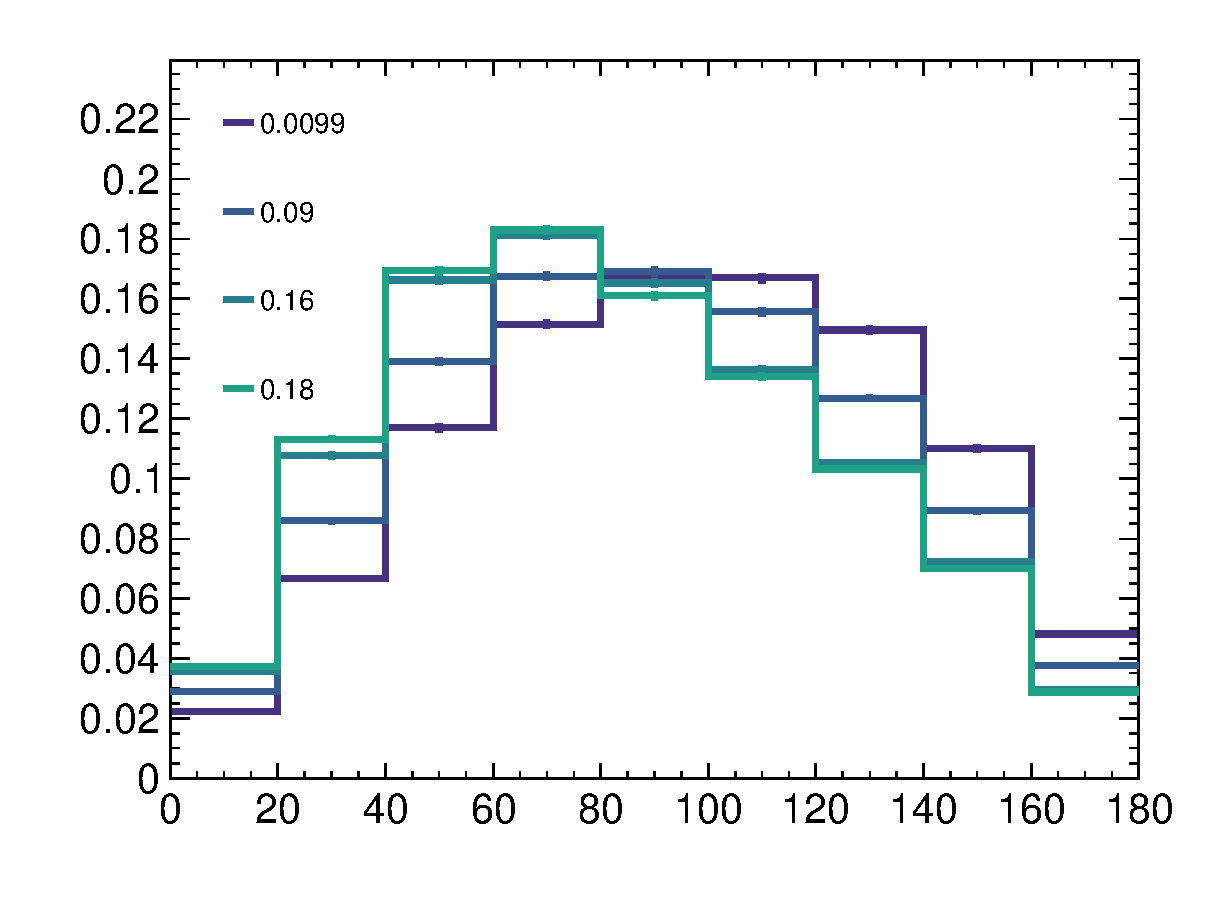
\includegraphics[width=\linewidth]{anorm-nuc-adt.eps}
    \caption{Anorm – Ermc comp (a) $\tp$ (b) $\adt$}
    \label{fig:ermc-comp}
\end{figure}


It is apparent in Fig.~\ref{fig:ermc-comp} that regardless of any changes in Ermc, $\tp$ is not affected at all. Meanwhile, there is a clear shift in the $\adt$ peak and a gradual change in its shape as well. This affirms the robust IS-independence of $\tp$ and the IS-dependence of $\adt$ as conjectured.
An additional desired property of $\ftp$ is its independence on the neutrino energy. As shown in Fig.~\ref{fig:enu-comp}. On the whole, the shapes of $\ftp$ for $\enu$ between $0.5\gev$ and $2.0\gev$ are largely similar over a large portion of the range. However, the deviation becomes larger at small angles. When $\enu$ increases to $5\gev$, the increase in the small angle region is apparent. It is likely due to the onset of the next doubly positive resonance. (which one?) If the selection is restricted to $\deltapp$, it is reassuring to see that the different curves collapse to one, demonstrating the independence from $\enu$. 

\begin{figure}
    \centering
    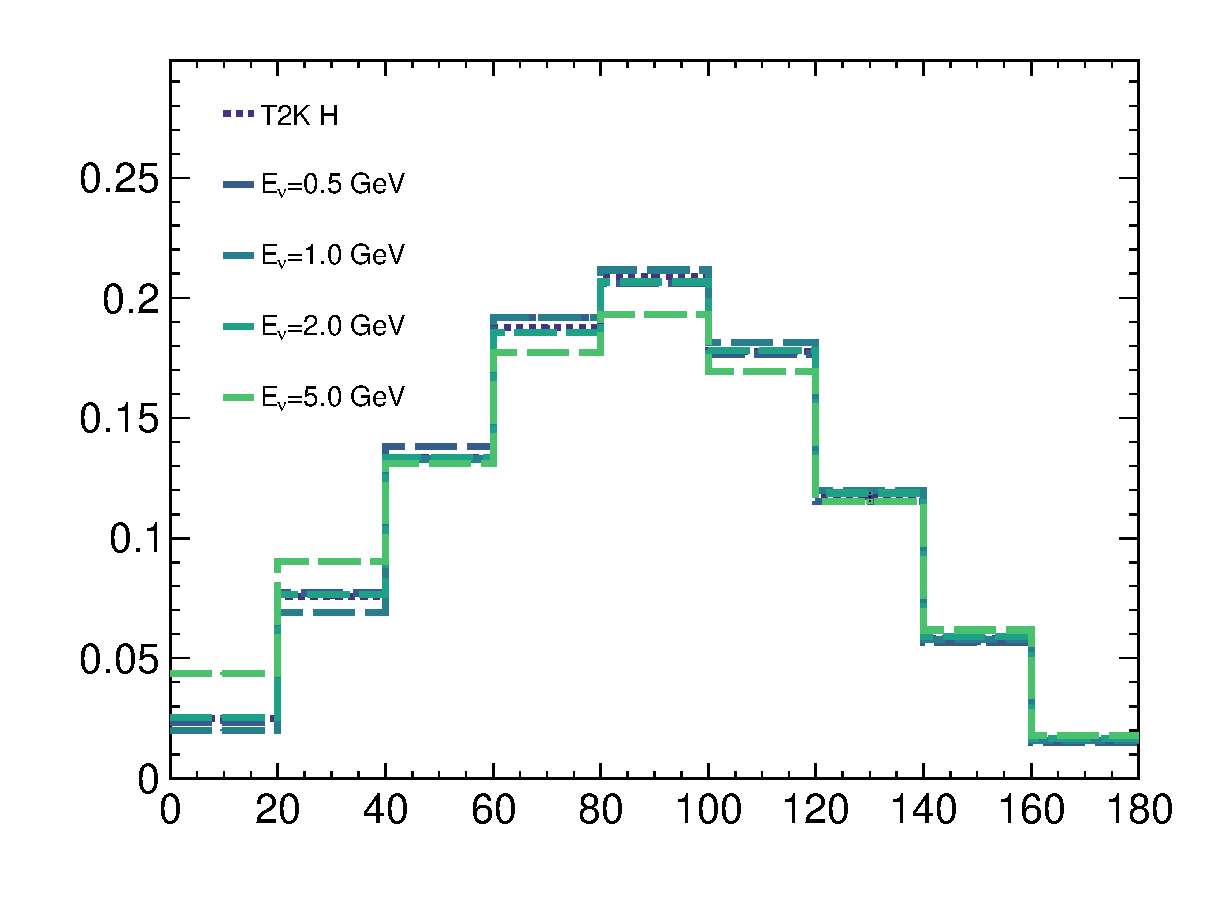
\includegraphics[width=\linewidth]{anorm-monoEnu-less-flux-da.eps}
    \caption{Anorm different enu fluxes ---- SHOULD PLOT ONE WITH MODE==11 ON FOR THE DIFFERENT ENU TO REMOVE HIGHER RESONANCE.}
    \label{fig:enter-label}
\end{figure}

\section{Discussion}
Through the multiple simulation studies, it has been demonstrated that the COM angle is a new variable with several strengths and its measurement will be valuable in studying FSI independently from IS. This discussion so far has focused on IS and FSI, but as $\deltapp$ is produced in RES, it is naturally affected by the modelling of $\nu$-N interaction. Fortunately, the $\nu$-N interaction is relatively better understood by directly studying $\nu$-H interactions. Hence, future RES modelling would not have drastically different predictions from the current one constrained by the bubble chamber data. To examine the impact of a change in the RES modelling on $\ftp$, the axial mass parameter is changed in steps. While it is expected that changing $MA$ will change the cross section, it is encouraging that the shape of $\ftp$ remains unchanged, as shown in Fig.~\ref{fig:ma-comp}. Hence, FSI models tuned using $\ftp$ will remain applicable even if the RES model is updated in the future, thereby enhancing the usefulness of an FSI model tuning. 

\begin{figure}
    \centering
    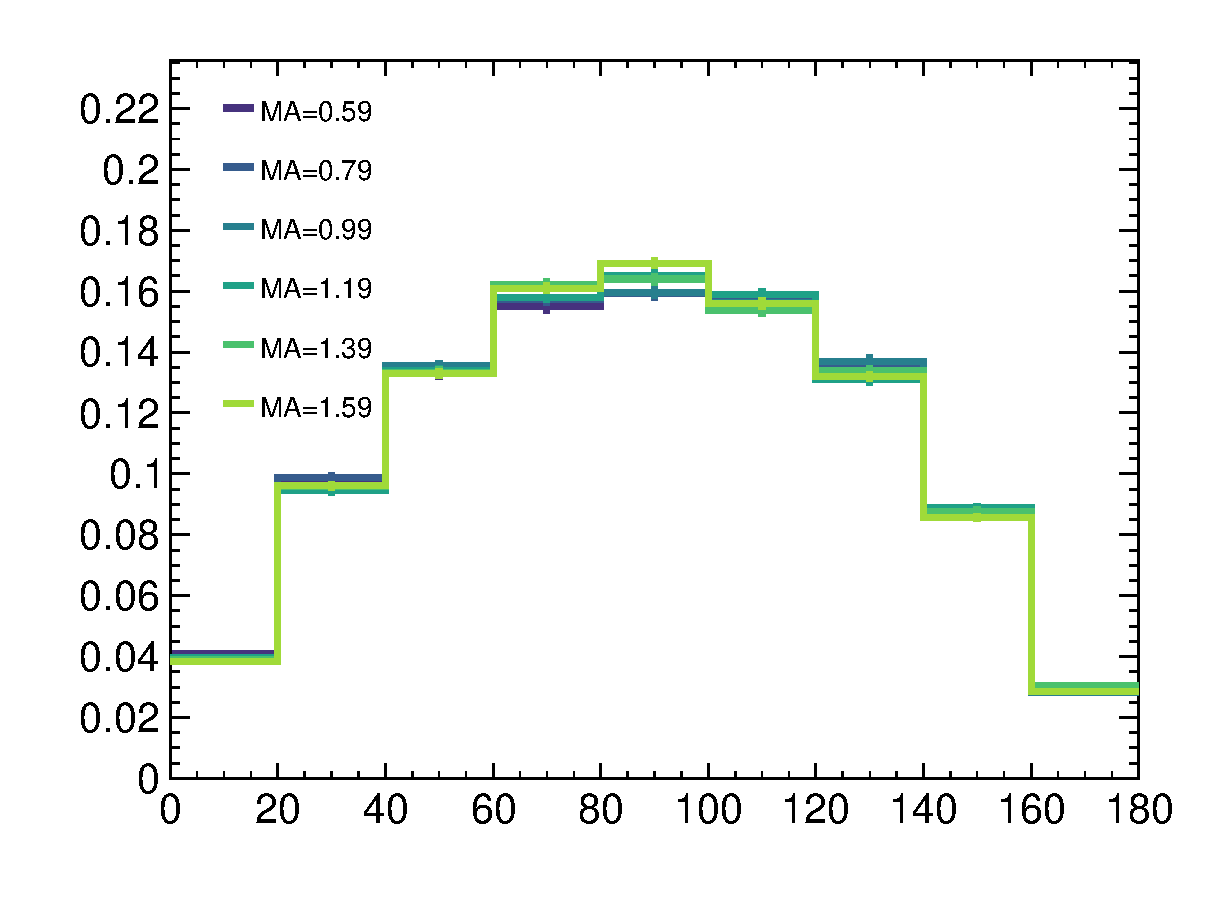
\includegraphics[width=\linewidth]{anorm-ma-da.eps}
    \caption{MA COMP xsec norm and anorm. }
    \label{fig:ma-comp}
\end{figure}

While $\ftp$ is relatively immune to change in $MA$, it might be affected considerably by added correlation between different resonances as hinted in the previous section in Fig.~\ref{fig:enu-comp}, where it is apparent that the next resonance has raised the low angle region of $\ftp$. As \genie does not handle resonance correlations, it will be interesting to study its impact in other generators in future works.
The sensitivity of the COM frame to FSI can not only be used to study FSI, but also to select events without FSI. These events are composed mainly of $\nu$-H interactions, which is the only venue to have a precise measurement of the axial current, unique to neutrinos. Moreover, a $\nu$-H sample offers the opportunity to further improve $\nu$-H modelling without the complications of IS and FSI, which additionally allows precise reconstruction of the neutrino energy. Its importance has sparked many efforts to invent techniques to select a high purity $\nu$-H sample, cite[dptt, Minerva, plong]. While Ref.~\cite[Min,plong] focuses on pion-less events, Ref.~\cite[dptt] is applicable to the same event topology of the COM total energy. A preliminary study has shown that a cut on COM E can cut away events with little transverse momentum imbalance, so it could be used in conjunction with cuts on $\dptt$ and $\dpt$ to produce a high purity $\nu$-H sample. It shall be studied in greater depth in future works.
While the COM angle has a similar reconstruction target as the Adler angle, they have important differences as shown in Sec.~\ref{sec:ana}. Although the difference might seem relatively small, the conceptual difference makes tuning FSI model using the COM angle more future-proof. Besides, the analyses presented are based on true information without smoothing, where difficulties and implications of reconstruction are absent, which can be significant for the neutrino energy required for the calculation of Adler angle. Hence, the full potential of the COM angle will be better demonstrated in a cross-section measurement that takes into consideration all of these complications.
\section{conclusion}
This work has introduced a new set of variables, the COM angle and total energy. They have multiple desired properties, thereby motivating cross section measurements of these variables, which could help to significantly improve our understanding and modelling of FSI in neutrino-nucleus interactions. 



\minitoc